\section{О физических и математических моделях металлических нанокластеров}
\label{sec:1}

Согласно определению, данному в [TODO] молекулярным кластером металлов называются
многоядерные комплексные соединения, в основе молекулярной структуры которых
находится окруженный лигандами остов из атомов металлов.

Физические модели кластеров могут быть основаны на квантовой или классической теории.
Квантовые неэмпирические подходы более адекватны, но их применение вызывает
большие сложности при построении математических моделей, а также при их
программировании. Выполнение программ, построенных на основе квантовых
неэмпирических подходов требует много машинного времени.

Ввиду этого большое распространение получили полуэмпирические подходы описания
межатомного взаимодействия, которые характеризуются аналитическими формулами,
содержащими подгоночные параметры. Такие формулы называются потенциальными
функциями взаимодействия или просто потенциалами. Примерами потенциальных функций
являются: потенциал Морзе, потенциал Леннарда--Джонса, потенциал Бакингема и др.

В настоящей работе используется потенциал Саттона--Чена, который применялся для
моделирования характеристик межатомного взаимодействия %TODO: Ссылка на статью.

Следующий подпараграф посвящен математическому формализму в рамках приближения
Саттона--Чена. Затем, в следующем подпараграфе, будет рассмотрен формализм метода
молекулярной динамики в режиме квазидинамического демпфирования. % Квазидинамическое демпфирование - что это?
В последнем подпараграфе (\ref{sec:1c}) описаны основные положения, которые
использовались при построении генетического алгоритма, который использовался в
диссертации.

\subsection{Потенциал Саттона--Чена}
\label{sec:1a}

При проведении экспериментов над пространственными структурами металлических кластеров
довольно часто используют потенциальную функцию Саттона--Чена (TODO: link to the article).
Полная потенциальная энергия при таком подходе рассчитывается следующим образом:
\begin{equation}
\label{Etot}
E_{tot}=\sum_i E_{i} = \sum_i \epsilon \left[\frac12\sum_{i\ne j} V(r_{ij})-c \sqrt{\rho_i}\right],
\end{equation}

Где
\begin{equation}
\label{V(r)}
V(r_{ij})=(a/r_{ij})^n,
\end{equation}

\begin{equation}
\label{p_i}
\rho_i=\sum_{i\ne j}\left(\frac{a}{r_{ij}}\right)^m
\end{equation}

Здесь $r_{ij}$  - раccтояние между атомами $i$ и $j$, $с$ - положительный
безразмерный параметр, $\epsilon$ - параметр, имеющий размерность энергии, $a$
- параметр длины, и $m$ и $n$ - положительные целые числа. По причинам, описанным
ниже, $n$ должно быть больше чем $m$. Парный потенциал, $V$, является просто
отталкивающим, и термин N-частичный просто связен. Обозначим значение $\rho^s$,
заданного суммой в равенстве (\ref{V(r)}) для атома, принадлежащего свободной
поверхности. Связный вклад, который этот атом делает к полной энергии
поверхности, таков $\epsilon=-\epsilon c \sqrt{\rho s}$. Если
дополнительный атом поместить выше поверхности и в разделение $R$ от нашего
поверхностного атома, значение $\rho^s$ изменяется на:
$$-\epsilon c[\rho^s+(a/R)^m]^{1/2}$$

Для больших значений $R$, по сравнению с $a$, мы можем расширить квадратный корень:
\begin{equation}
\label{R4}
[\rho^s+(a/R)^m]^{1/2}\backsimeq \sqrt{\rho s}+ \frac{(a/R)^m}{2\sqrt{\rho s}}
\end{equation}

Из выражения (\ref{R4}) видно, что когда атом приближается к поверхности, он
взаимодействует в больших разделениях попарным способом, хотя величина этого
парного потенциала зависит от числа соседей каждого поверхностного атома. Как
разделение, $R$, уменьшается, расширение в выражении (\ref{R4}) становится все
более и более недействительным, и взаимодействие гладко изменяется на
N-частичную форму. Таким образом, выбирая $m$=6 в выражении (\ref{p_i}), мы можем
достигнуть нашей цели взаимодействий дальнего действия между двумя группами
атомов, описываемых парным потенциалом $1/r^6$, тогда как в маленьких
разделениях N-частичное взаимодействие в природе. Кроме того, переход между
этими двумя пределами гладкий и непрерывный.

% TODO: Table with parameters of different metals parameters? 

\subsection{Формализм метода молекулярной динамики}
\label{sec:1b}

Метод молекулярной динамики~--- метод, в котором временная эволюция системы
взаимодействующих атомов или частиц отслеживается интегрированием их уравнений
движения.

Концептуально классическая молекулярная динамика включает:

1. решение уравнений движения Ньютона для взаимодействующих атомов или молекул;

2. статистический анализ полученных траекторий в фазовом пространстве системы.

Пусть некоторая система состоит из n атомов и известна их потенциальная энергия
взаимодействия $U(r_1, r_2, \cdots , r_n).$
Согласно уравнению движения классической механики:
\begin{equation}
\label{one}
m_{i}a_{i}=f_i=-\frac{\partial}{\partial r_i}U,
\end{equation}
для каждого атома $i$ можно найти его траекторию $r_i(t)$. Здесь $m_i$ - масса
атома, $a_i=\partial^2r_i/\partial t^2$ - ускорение,
$f_i$ - сила, действующая на атом $i$ со стороны остальных атомов. При
известных начальных условиях для координат $r_i(0)=r_i^0$ и
скоростей $\upsilon_i(0)=\upsilon_i^0$  задача является
детерминистической, то есть временная эволюция координат $r_i(t)$
однозначно определена. Таким образом, в компьютере можно проследить "жизненный
путь" всех атомов в системе. Например, непосредственно увидеть процесс
встраивания в пленку атома, осаждаемого из газа; развитие каскада атомных
соударений при внешнем облучении; распространение трещины при разрушении;
образование зародышей новой фазы; детали атомных перестроек в жидкости и другие
явления, которые иным способом исследовать либо трудно, либо невозможно.

При изучении макроскопических свойств системы сами по себе траектории атомов
$r_i(t)$ не представляют особого интереса. Они используются для
нахождения плотности вероятности заполнения фазового пространства системы.
Траектории атомов дают набор конфигураций, распределенных в соответствии с
некоторым статистическим ансамблем. В этом смысле метод молекулярной динамики является
методом статистической механики, которая прокладывает мостик между микроскопическим
поведением и термодинамикой.

Применимость уравнений движения классической механики (\ref{one}) для атомарных
систем имеет известные ограничения. Длина волны де Бройля $\lambda$ должна быть
меньше среднего межатомного расстояния а :
\begin{equation}
\label{two}
\lambda \ll a, \lambda=\sqrt{2\pi\hbar/m\kappa_B T},
\end{equation}
здесь $T$ - температура, $\kappa_B$ - постоянная Больцмана. Соотношение
(\ref{two}) нарушается для легких атомов, таких как $H$, $He$. Кроме того,
квантовые эффекты становятся существенными при низких температурах для любых
атомарных систем, что следует учитывать при интерпретации результатов, полученных
методом молекулярной динамики, в этой температурной области.

В методе молекулярной динамики силы находятся из потенциальной энергии системы
U (\ref{one}). Можно сказать, что правильный выбор потенциальной энергии
межатомного взаимодействия является ключевым элементом всего метода
молекулярной динамики. Как уже было сказано в параграфе \ref{sec:1a}, в данной
работе был использован потенциал Саттона--Чена.

Метод молекулярной динамики позволяет найти глобальный минимум потенциальной энергии
многоатомной системы. В то время как различные подходы минимизации потенциальной энергии
системы по координатам ядер этого не гарантируют.

\subsection{Генетический алгоритм}
\label{sec:1c}

Использование генетического алгоритма для оптимизации кластерных структур
началось в 90-х годах с работ Хартке (для кремниевых кластеров малого размера)
\cite{Hartke1993} и Вильямса (для молекулярных кластеров) \cite{Xiao1993}. В обоих
случаях структура кластеров была закодирована с помощью бинарных строк. При этом
генетические операторы использовали бинарные операции над ними. Важным улучшением
генетического алгоритма для кластерной оптимизации стало использование действительных
Декартовых координат для представления кластеров. Этот подход был предложен
Зейри \cite{Zeiri1995} и позволил снять ограничение на бинарное кодирование генов.

Следующий шаг в развитии генетических алгоритмов для кластерной оптимизации был
предложен Дивеном и Хо \cite{Deaven1995}. Главной идеей является нахождение локального
минимума общей потенциальной энергии кластера для каждого кластера, полученного
с помощью генетического алгоритма на очередном шаге. Это позволяет значительно
уменьшить пространство возможных решений для генетического алгоритма.

Дивен и Хо также предложили трехмерный оператор скрещивания, которую назвали
"разрез и склеивание" ("cut and splice"). Этот оператор, который использовался
в большинстве последующих работ по кластерной оптимизации, привносит больше 
физического значения в процесс скрещивания. Этот механизм будет описан более
подробно позже.

На основе вышеперечисленных разработок в области генетических алгоритмов для
кластерной оптимизации Джонстон и др. предложили генетический алгоритм,
который назвали "Бирмингемским" \cite{Johnston2002}. Именно этот алгоритм и был
выбран при реализации экспериментального программного обеспечения.
Основные особенности этого алгоритма описаны ниже:

{\subsubsection Инициализация}.
Для кластера заданного размера (состоящего из $N$ элементов) генерируется $N_{clus}$
(значение по умолчанию - 20) кластеров случайным образом для формирования начальной
популяции.

{\it Функция приспособленности}

Функция приспособленности конкретной особи это оценка качества особи с точки зрения
конкретной задачи. В данном случае, кластеры с наименьшей энергией (наименьшей $V_{clus}$)
имеют наибольшее значение функции приспособленности. Генетический алгоритм использует
динамическое масштабирование приспособленности, основанное на нормализованном значении
энергии, $\rho$:

\begin{equation}
  \rho_{i} = \frac{V_{i} - V_{min}}{V_{max}-V_{min}}
\end{equation}

где $V_{min}$ и $V_{max}$ минимальное и максимальное значение энергии кластеров в
текущей популяции соответственно.

{\bf Скрещивание}

Родители для скрещивания выбираются с помощью "турнирного" метода. Несколько кластеров
выбираются случайным образом, чтобы образовать "турнирную" группу. Два кластера с минимальной
энергией затем выбираются из этой группы в качестве родителей. При такой схеме кластеры
с наибольшим значением функции приспособленности имеют высокую вероятность быть выбранными
для скрещивания и таким образом передать особенности своей структуры следующим поколениям.

Используемая процедура скрещивания представляет собой вариант оператора "разрез и склеивание",
предложенного Дивеном и Хо \cite{Deaven1995}. К кластерным структурам обоих родителей сначала
применяются случайные повороты вокруг двух перпендикулярных осей, а затем оба кластера разрезаются
горизонтально параллельно плоскости $xy$ посередине и соответствующие части склеиваются вместе,
как показано на рис. \ref{cut_and_splice}.

В результате процедуры скрещивания появляется один новый потомок. "Турнирный метод" применяется
столько раз, сколько потомков необходимо получить в следующем поколении.
Для каждый кластера-потомка затем применяется градиентный метод, чтобы структура кластера
соответствовала ближайшему локальному минимуму потенциальной энергии.

\begin{figure}[h!]
\centering
  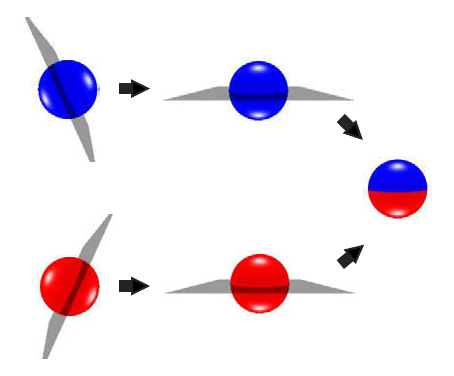
\includegraphics[width=0.5\textwidth]{./FIGs/cut_and_splice.png}
\caption{Оператор скрещивания "разрез и склеивание"}
\label{cut_and_splice}
\end{figure}

{\bf Мутация}

Несмотря на то, что операция скрещивания приводит к перемешиванию генетического материала
в кластерах-потомках, нового генетического материала при этом не появляется. Для того, чтобы
поддержать разнообразие особей в популяции, вводится новый оператор мутации. Каждая особь
имеет некоторую вероятность подвергнуться мутации ($P_{mut}$), которая возмущает некоторые или
все позиции атомов внутри кластера. После мутации, каждая особь локально минимизируется.

Может быть использовано несколько видов мутации:

\begin{itemize}
  \item{\bf Перемещение атомов} {Данная мутация заменяет координаты некоторых атомов кластера
случайными значениями. Количество атомов для замены координат было выбрано равным
трети ($N/3$) от общего количества атомов.}
\item{\bf Вращение} Происходит поворот верхней части кластера вокруг оси $z$ на случайный угол
относительно нижней части кластера.
\item{\bf Замена кластера} Происходит замена целого кластера на новый, координаты которого заданы
случайным образом. 
\end{itemize}

Перечисленные мутации приводят к достаточно значительным изменениям генетического материала.


{\bf Последующие популяции}

Новая популяция представляет собой объединение некоторого количества ($N_{clus}$) кластеров
с большими значениями функции приспособленности, некоторого количества потомков ($N_{off}$),
а также некоторого количества мутировавших кластеров.

Процесс последовательного скрещивания, мутации и селекции происходит заданное количество
раз ($N_{gen}$).

\subsection{Технологии визуализации результатов расчета}
\label{sec:1d}

Построение равновесной пространственной конфигурации для нанокластера
предполагает нахождение координат всех атомов кластера. Так как количество
атомов в кластере может быть достаточно большим, то необходимо визуальное
представление полученной пространственной конфигурации для помощи в последующих
исследованиях этой конфигурации. Для визуализации результатов были опробованы
два инструмента: библиотека для построения графиков DISLIN, а также
молекулярный редактор и визуализатор Avogadro.

% TODO: Insert links to tools websites to literature
DISLIN является бесплатной кросс-платформенной высокоуровневой библиотекой для
построения графиков, доступной для нескольких языков программирования (C,
Fortran, Java, Ruby, Python).  Библиотека предоставляет небольшое количество
функций непосредственно построения графиков с коротким списком параметров, а
также большое количество функций для детальной настройки различных параметров
отображения графиков.

Пример графика, построенного с помощью библиотеки DISLIN во время изучения её 
возможностей, показан на рис. \ref{DISLIN_picture}. Преимуществами библиотеки
являются простой и понятный интерфейс прикладного программирования, а также
большое количество поддерживаемых графических форматов для вывода результатов,
как векторных, так и растровых.

\begin{figure}[ht!]
\centering
  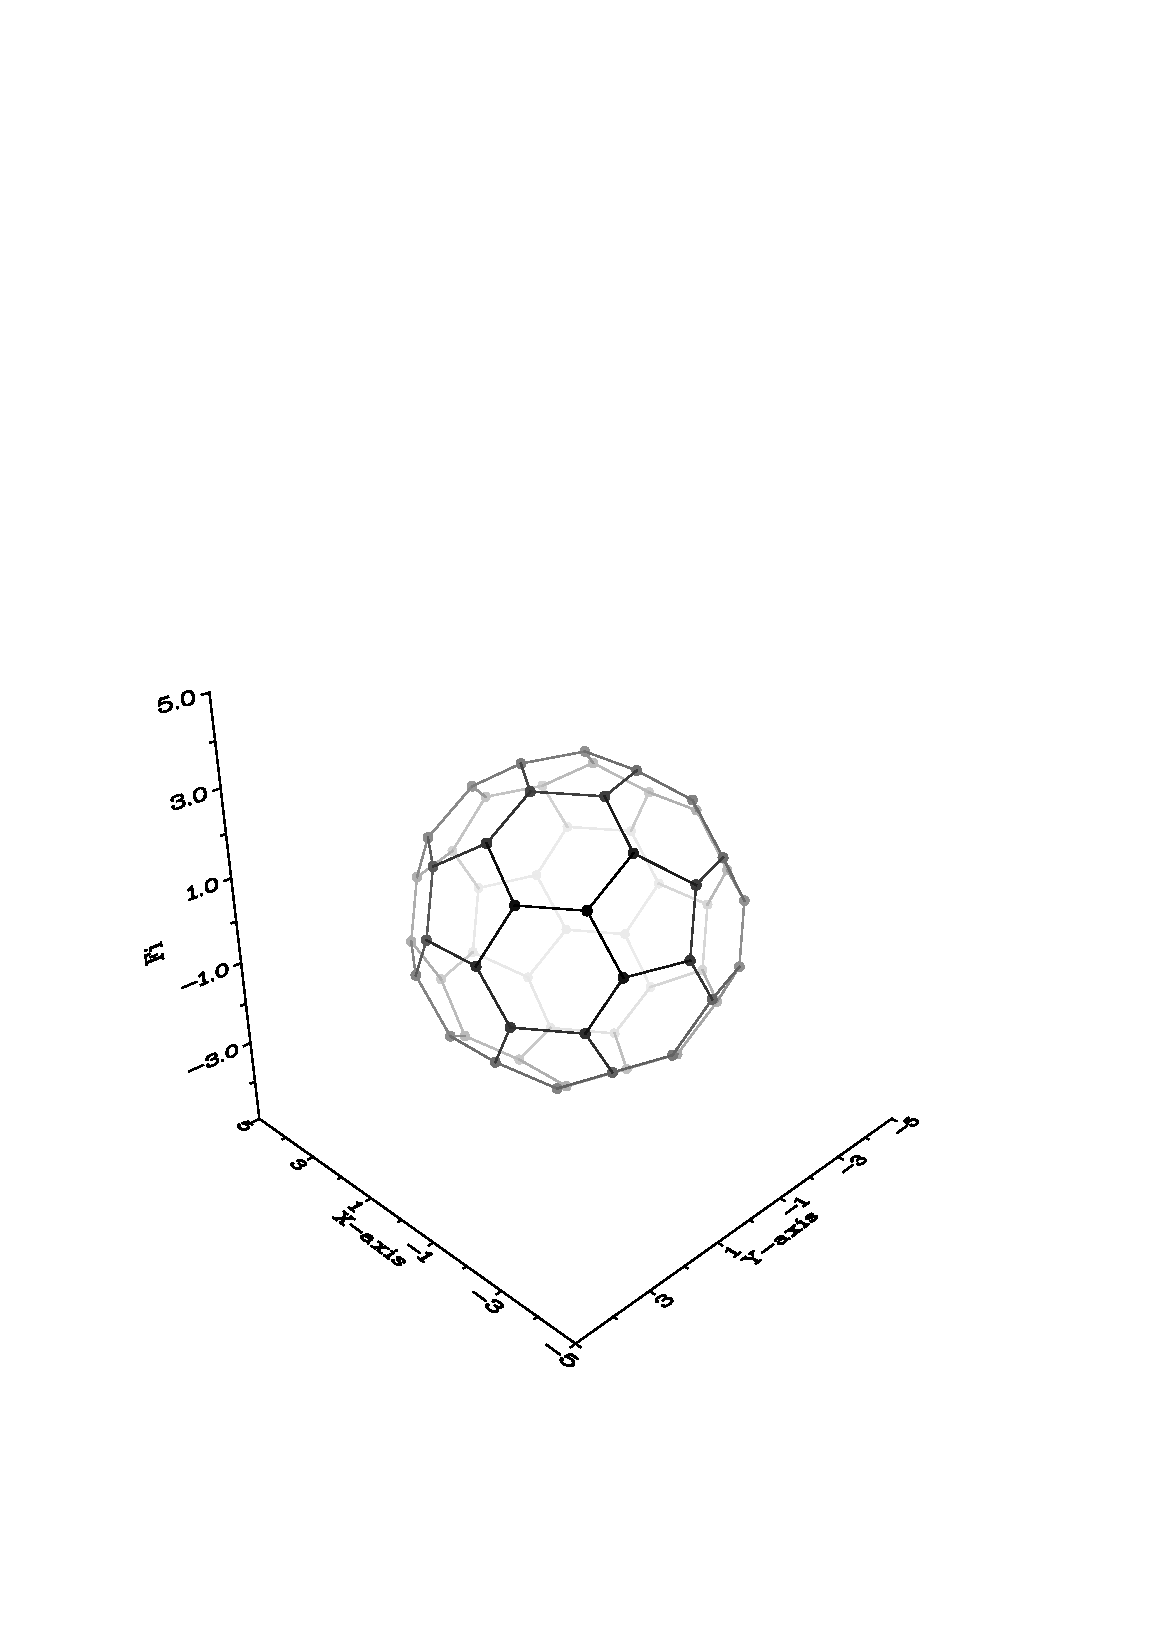
\includegraphics[trim=30 120 30 330, clip, width=0.8\textwidth]{./FIGs/DISLIN_fullerene.pdf}
\caption{Фуллерен $C_{60}$, построенный с помощью библиотеки DISLIN}
\label{DISLIN_picture}
\end{figure}

Вторым рассмотренным вариантом для визуализации результатов является молекулярный
редактор и визуализатор Avogadro. Avogadro является открытым и кросс-платформенным
программным обеспечением. Он позволяет моделировать различные химические
соединения, используя графический редактор. В качестве формата файлов для хранения
построенных моделей используется формат CML (Chemistry markup language).

Для создания и редактирования формата CML из прикладной программы существует библиотека
Open Babel. Open Babel представляет собой открытый набор утилит и библиотек для работы с
химическими данными, представленными в различных форматах. Используя библиотеку Open Babel
возможно в том числе манипулировать данными в формате CML, не вдаваясь в подробности
реализации хранения данных, а работая с такими высокоуровневыми абстракциями как молекулы и
химические связи. Пример визуального отображения модели фуллерена $C_{60}$, хранящейся в формате
CML и открытой для редактирования в приложении Avogadro представлен на рис. \ref{Avogadro_screenshot}.

\begin{figure}[ht!]
\centering
  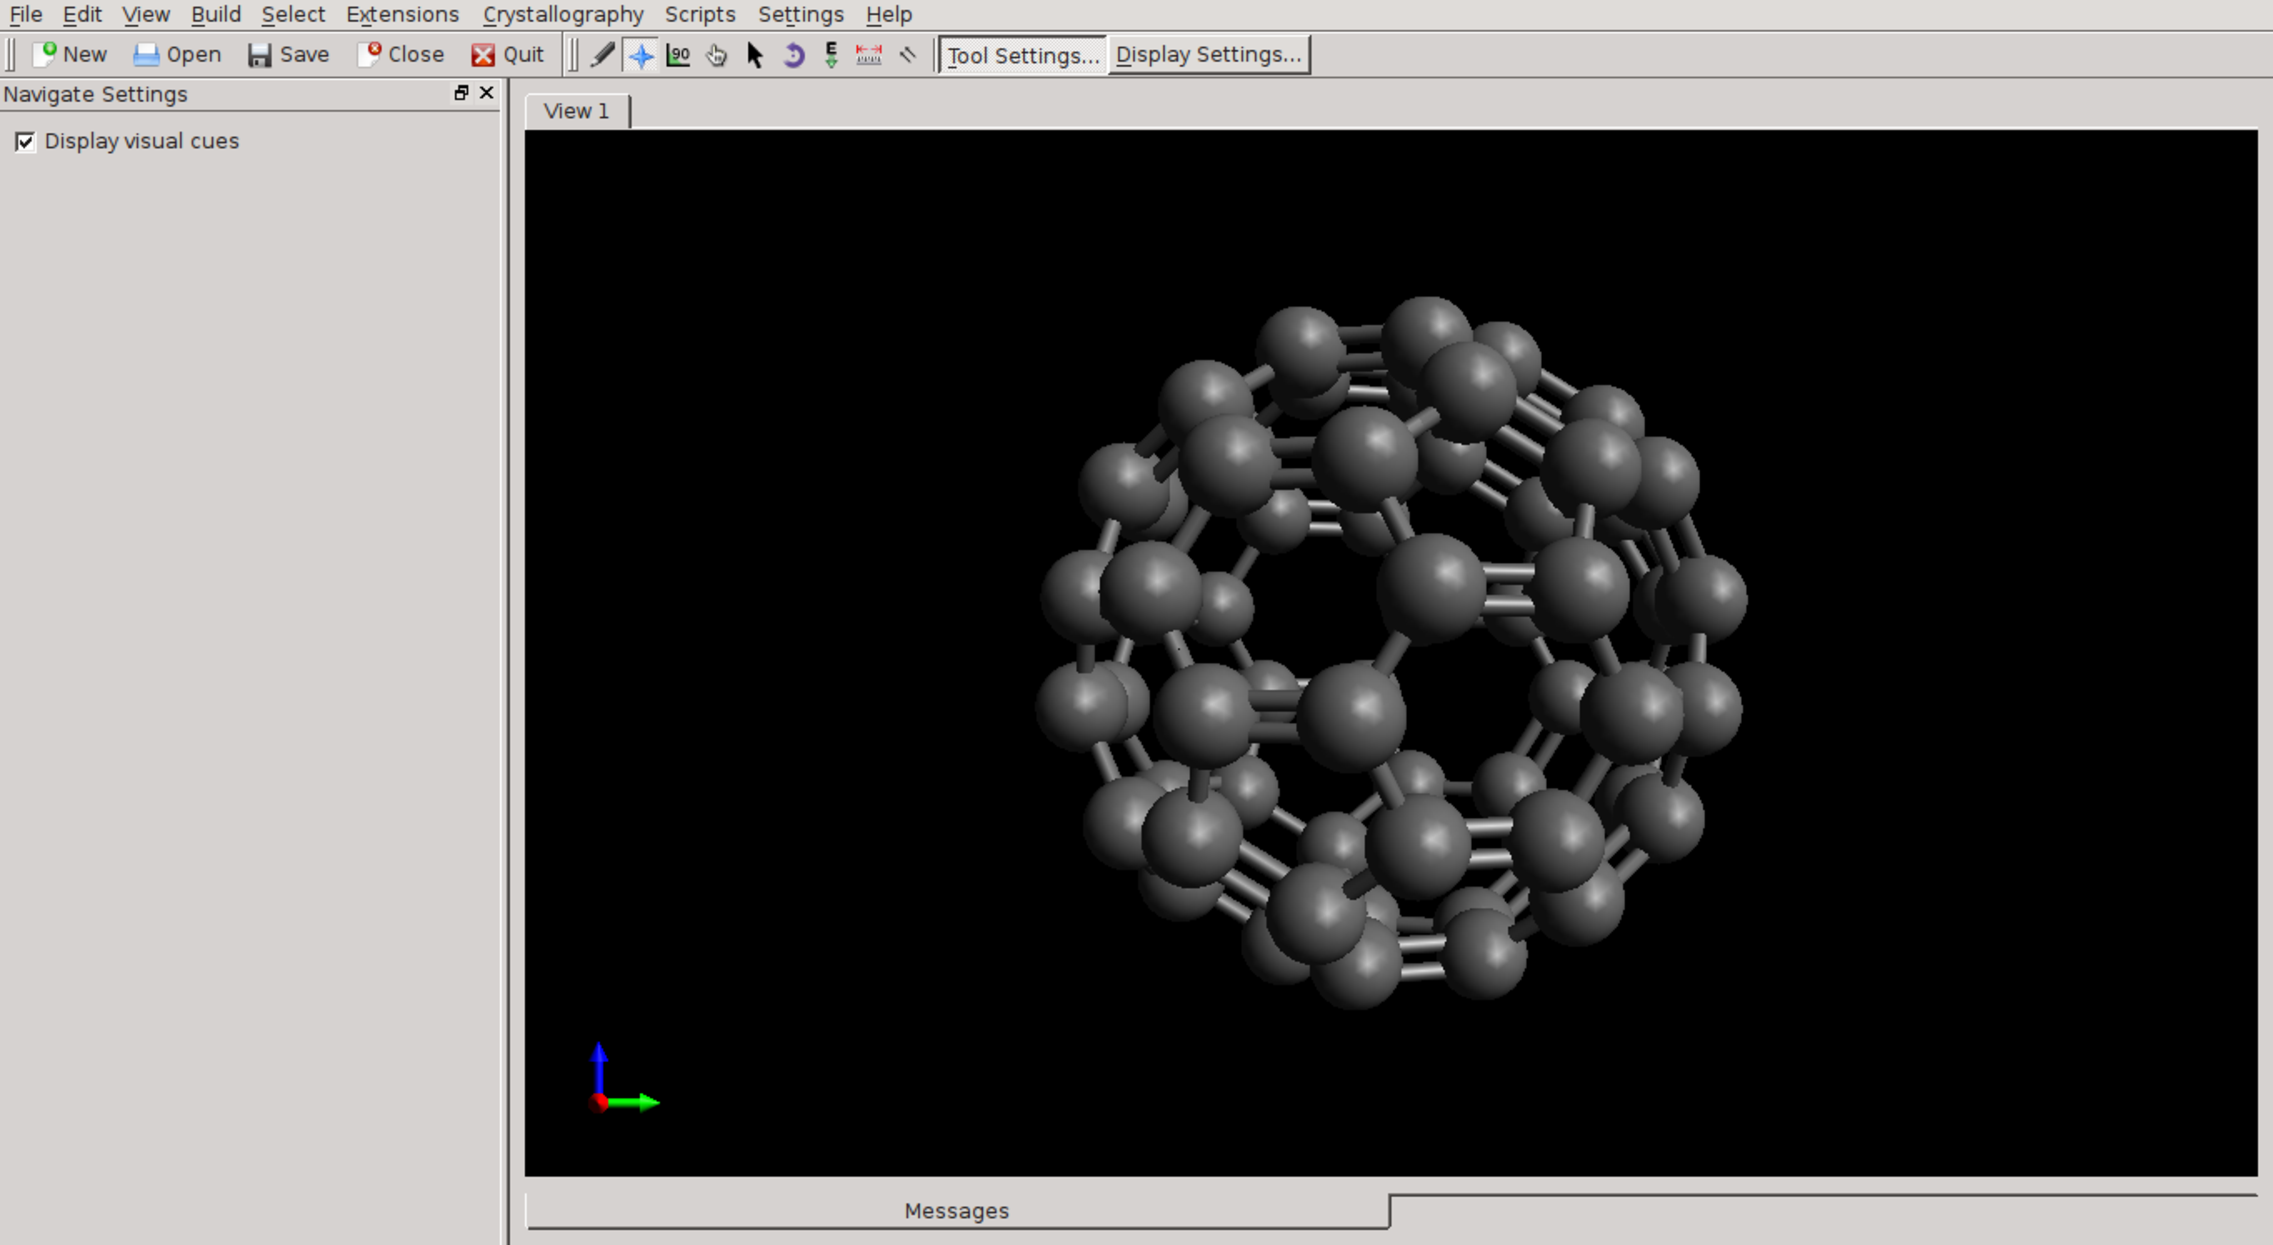
\includegraphics[width=1.0\textwidth]{./FIGs/Avogadro_screenshot.pdf}
\caption{Модель фуллерена $C_{60}$, открытая в приложении Avogadro}
\label{Avogadro_screenshot}
\end{figure}

Главным преимуществом использования формата CML для представления пространственной
конфигурации нанокластера перед использованием библиотеки DISLIN является последующее
удобство работы и редактирования этой конфигурации, используя приложение Avogadro.
Поэтому, в данной работе для визуализации получаемых пространственных конфигураций
были использованы библиотека Open Babel и приложение Avogadro.

